\documentclass[11pt]{beamer}
\usepackage[utf8]{inputenc}
\usepackage[T1]{fontenc}
\usepackage{lmodern}
\usepackage[czech]{babel}
\usetheme{metropolis}
\begin{document}
	\author{Lukáš Růžička}
	\title{Svobodný software}
	\subtitle{právo na svobodu počítačování}
	%\logo{}
	\institute{lruzicka@redhat.com}
	\date{září 2020}
	%\subject{}
	%\setbeamercovered{transparent}
	%\setbeamertemplate{navigation symbols}{}
	\begin{frame}[plain]
		\maketitle
	\end{frame}

	\begin{frame}{Svoboda}
	 \begin{center}
	 	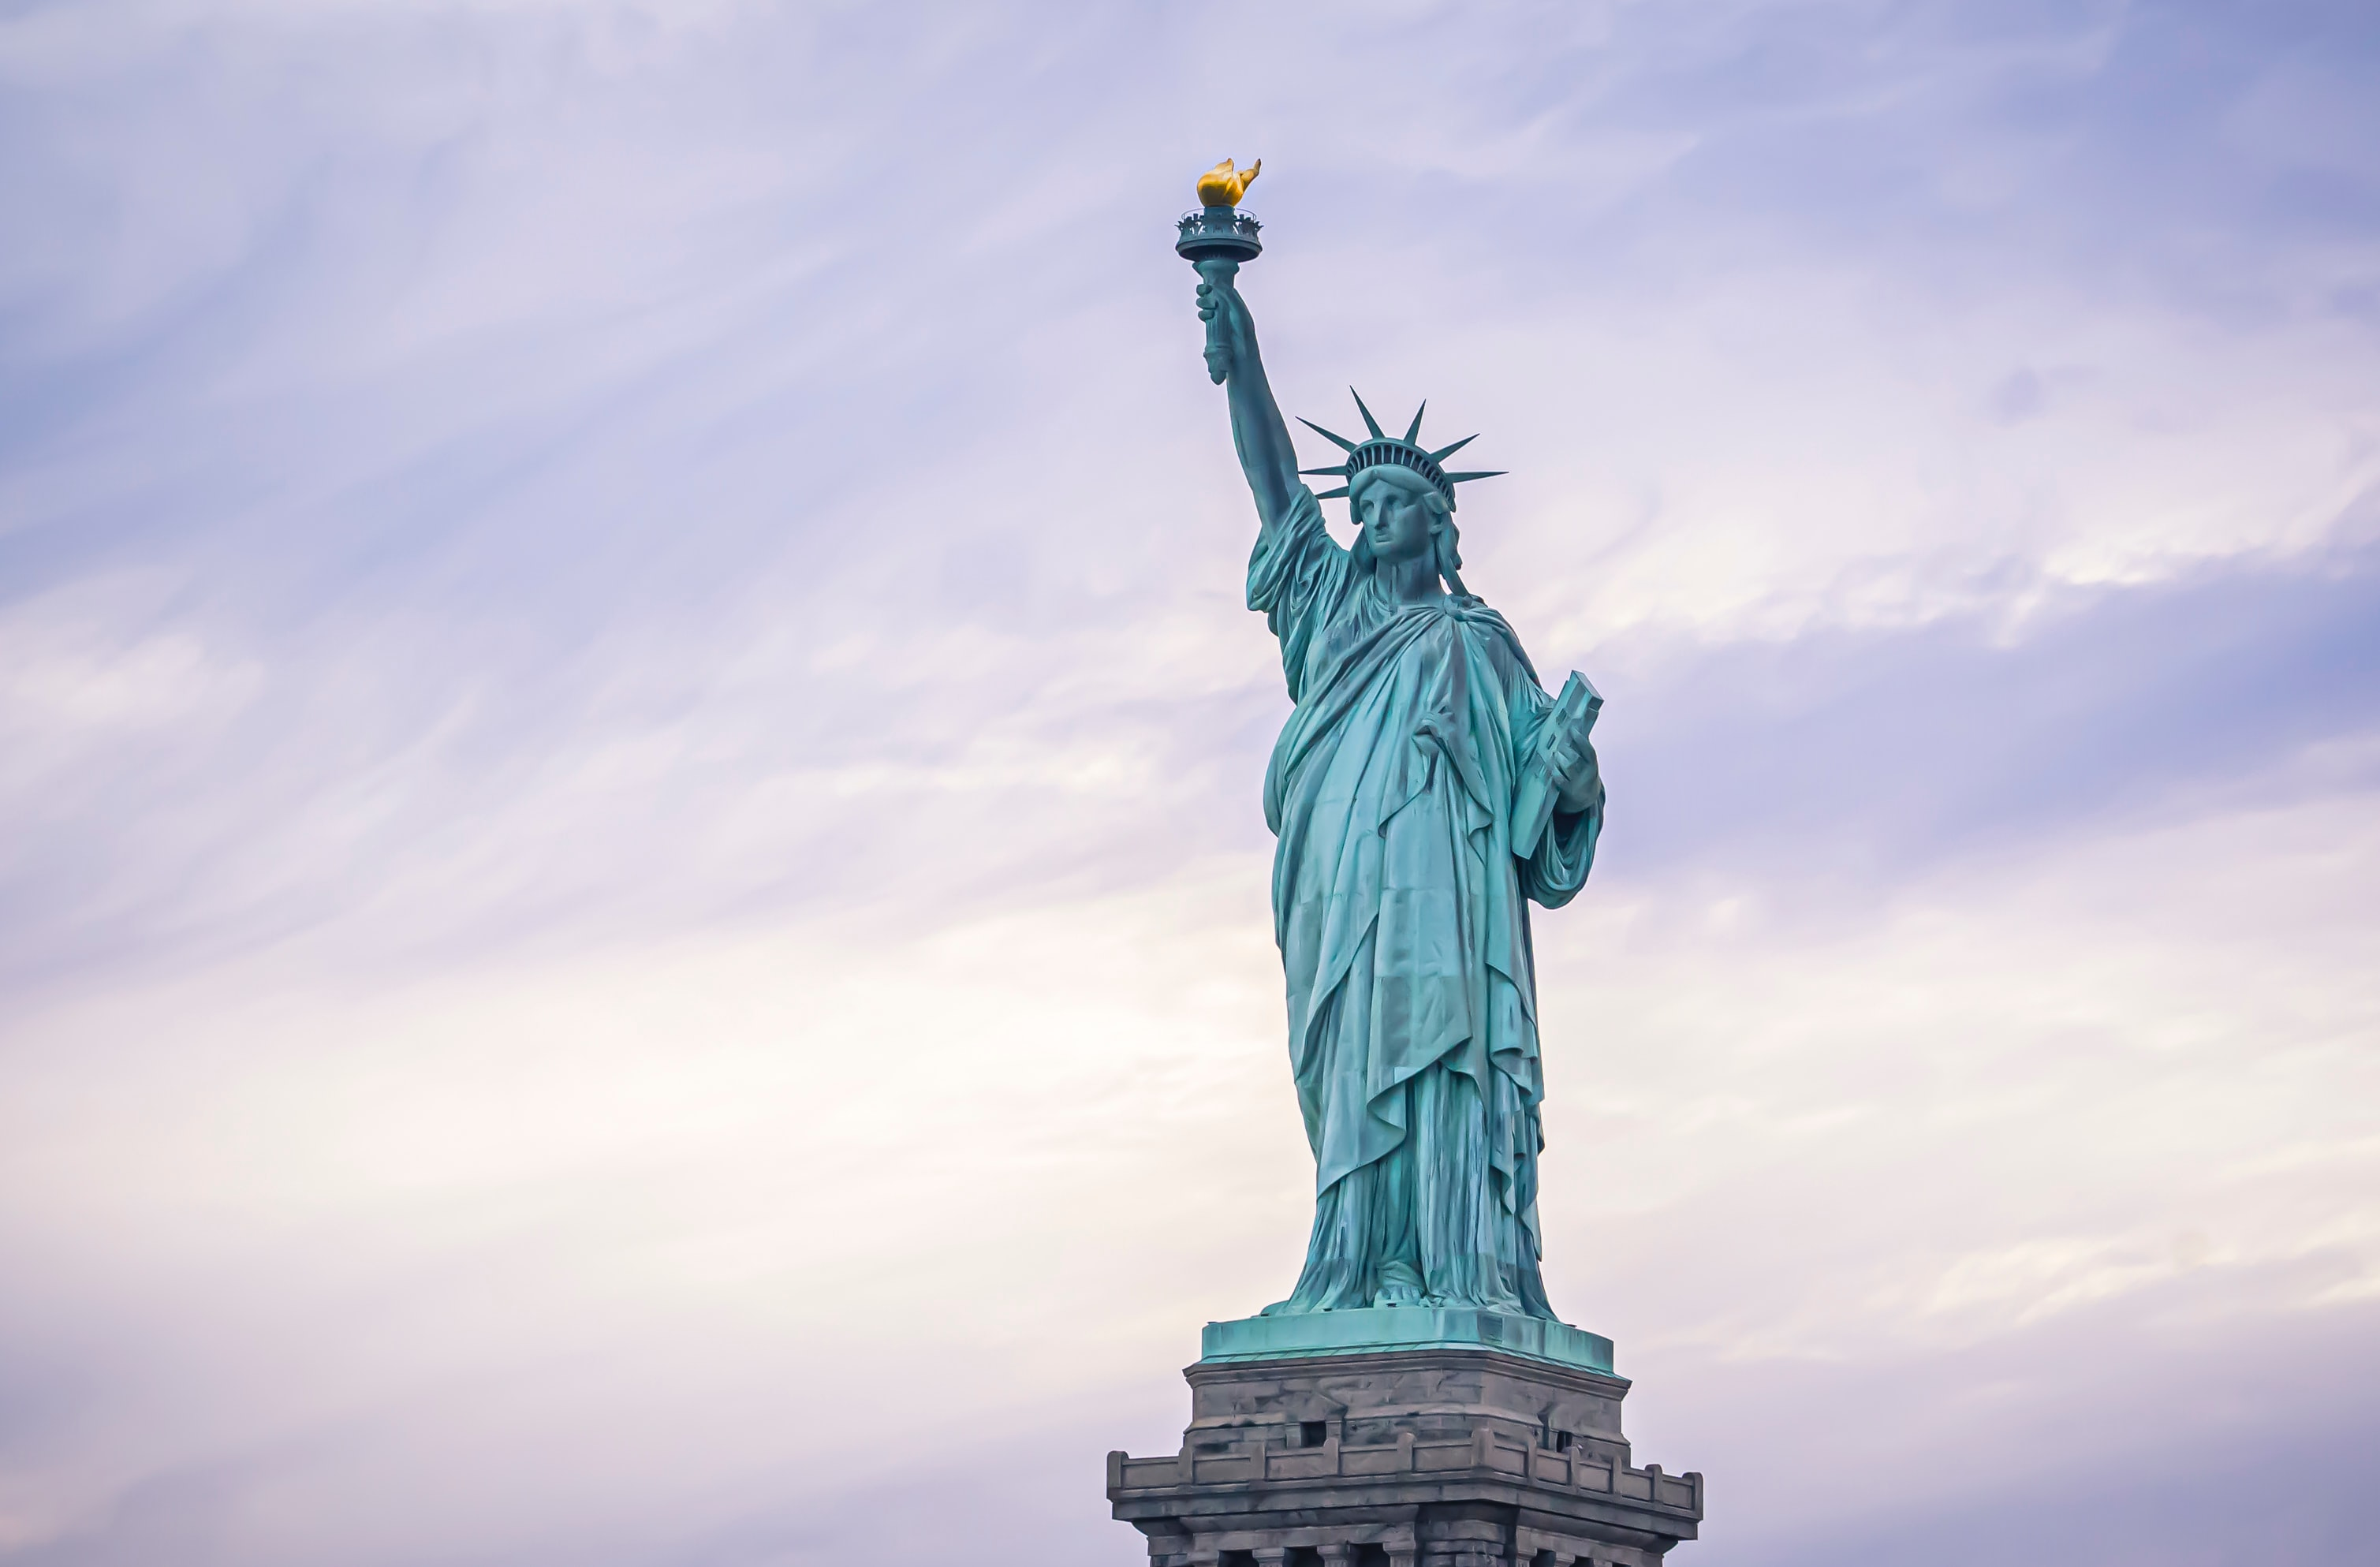
\includegraphics[width=\textwidth]{images/statue_of_liberty.jpg}
	 \end{center}
     \begin{flushright}
     	\textit{(Freddy-G)}
     \end{flushright}
 
	\end{frame}

	\begin{frame}{Co je svoboda?}
		\begin{quote}
			\textbf{Svoboda} je možnost, případně také schopnost, volit, rozhodovat a jednat \uv{podle své vůle}, ať je jakákoli a nést za to přiměřenou odpovědnost.\footnote{https://cs.wikipedia.org/wiki/Svoboda} 
		\end{quote}
	\end{frame}
	
	\begin{frame}{Důležitost svobody}
	\begin{columns}
		\begin{column}{0.5\textwidth}
			\begin{quote}
				Ten, kdo se ve jménu bezpečnosti vzdává svobody, nezaslouží si ani svobodu ani bezpečnost.
			\end{quote}
			\begin{flushright}
				(Benjamin Franklin)
			\end{flushright}
		\end{column}
		\begin{column}{0.5\textwidth}
			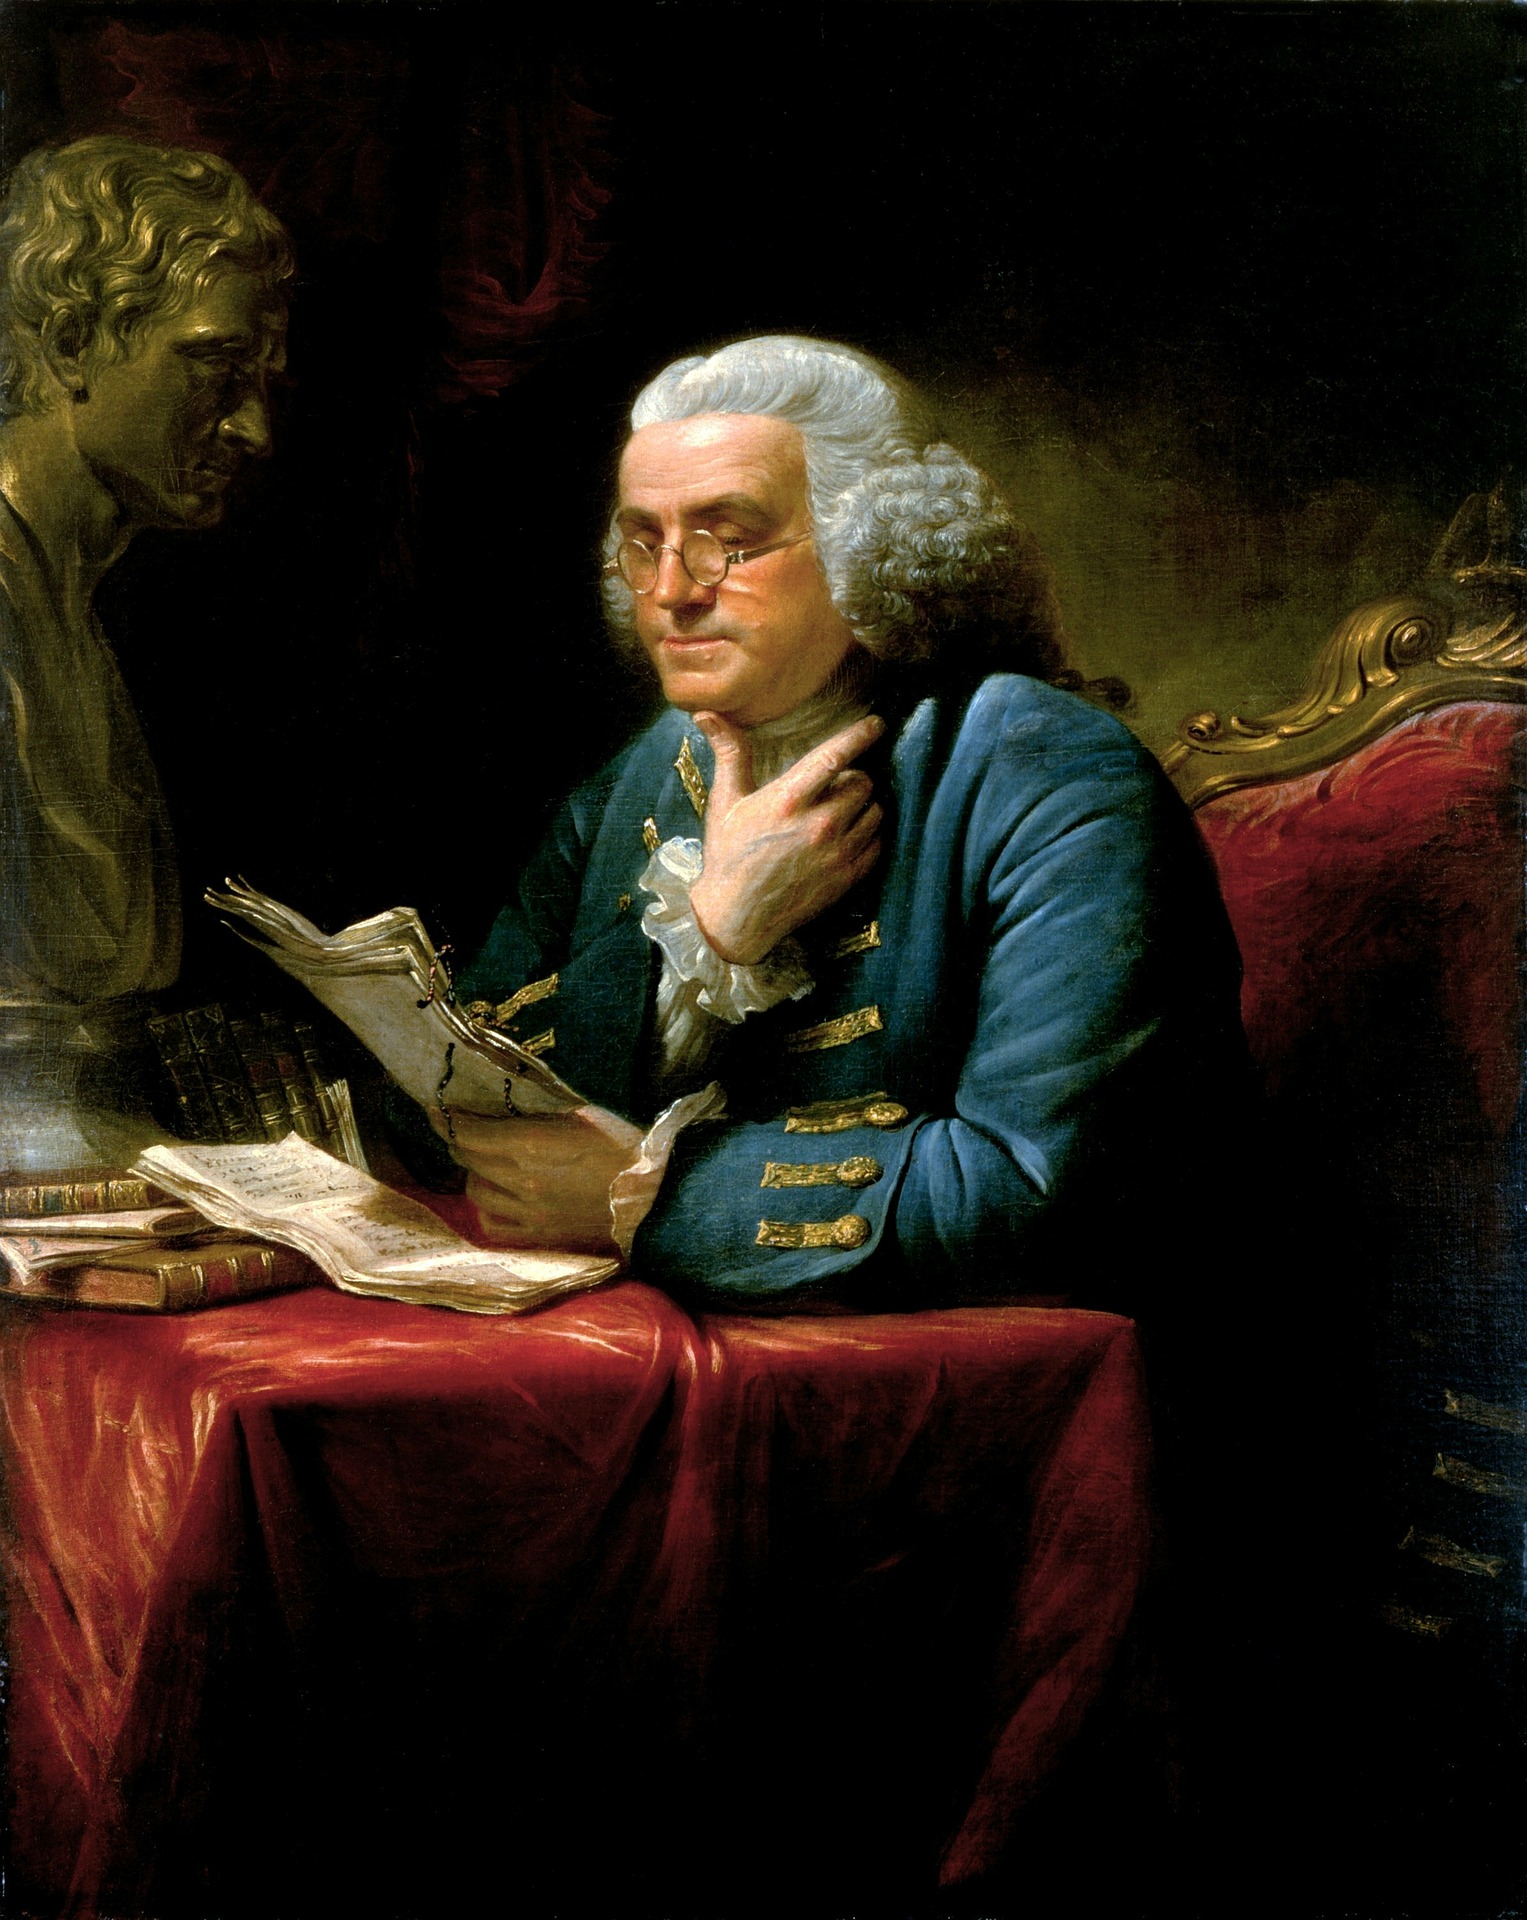
\includegraphics[width=5cm]{images/franklin.jpg}
		\end{column}
	\end{columns}
	\end{frame}

	\begin{frame}{Historie}
	\begin{center}
		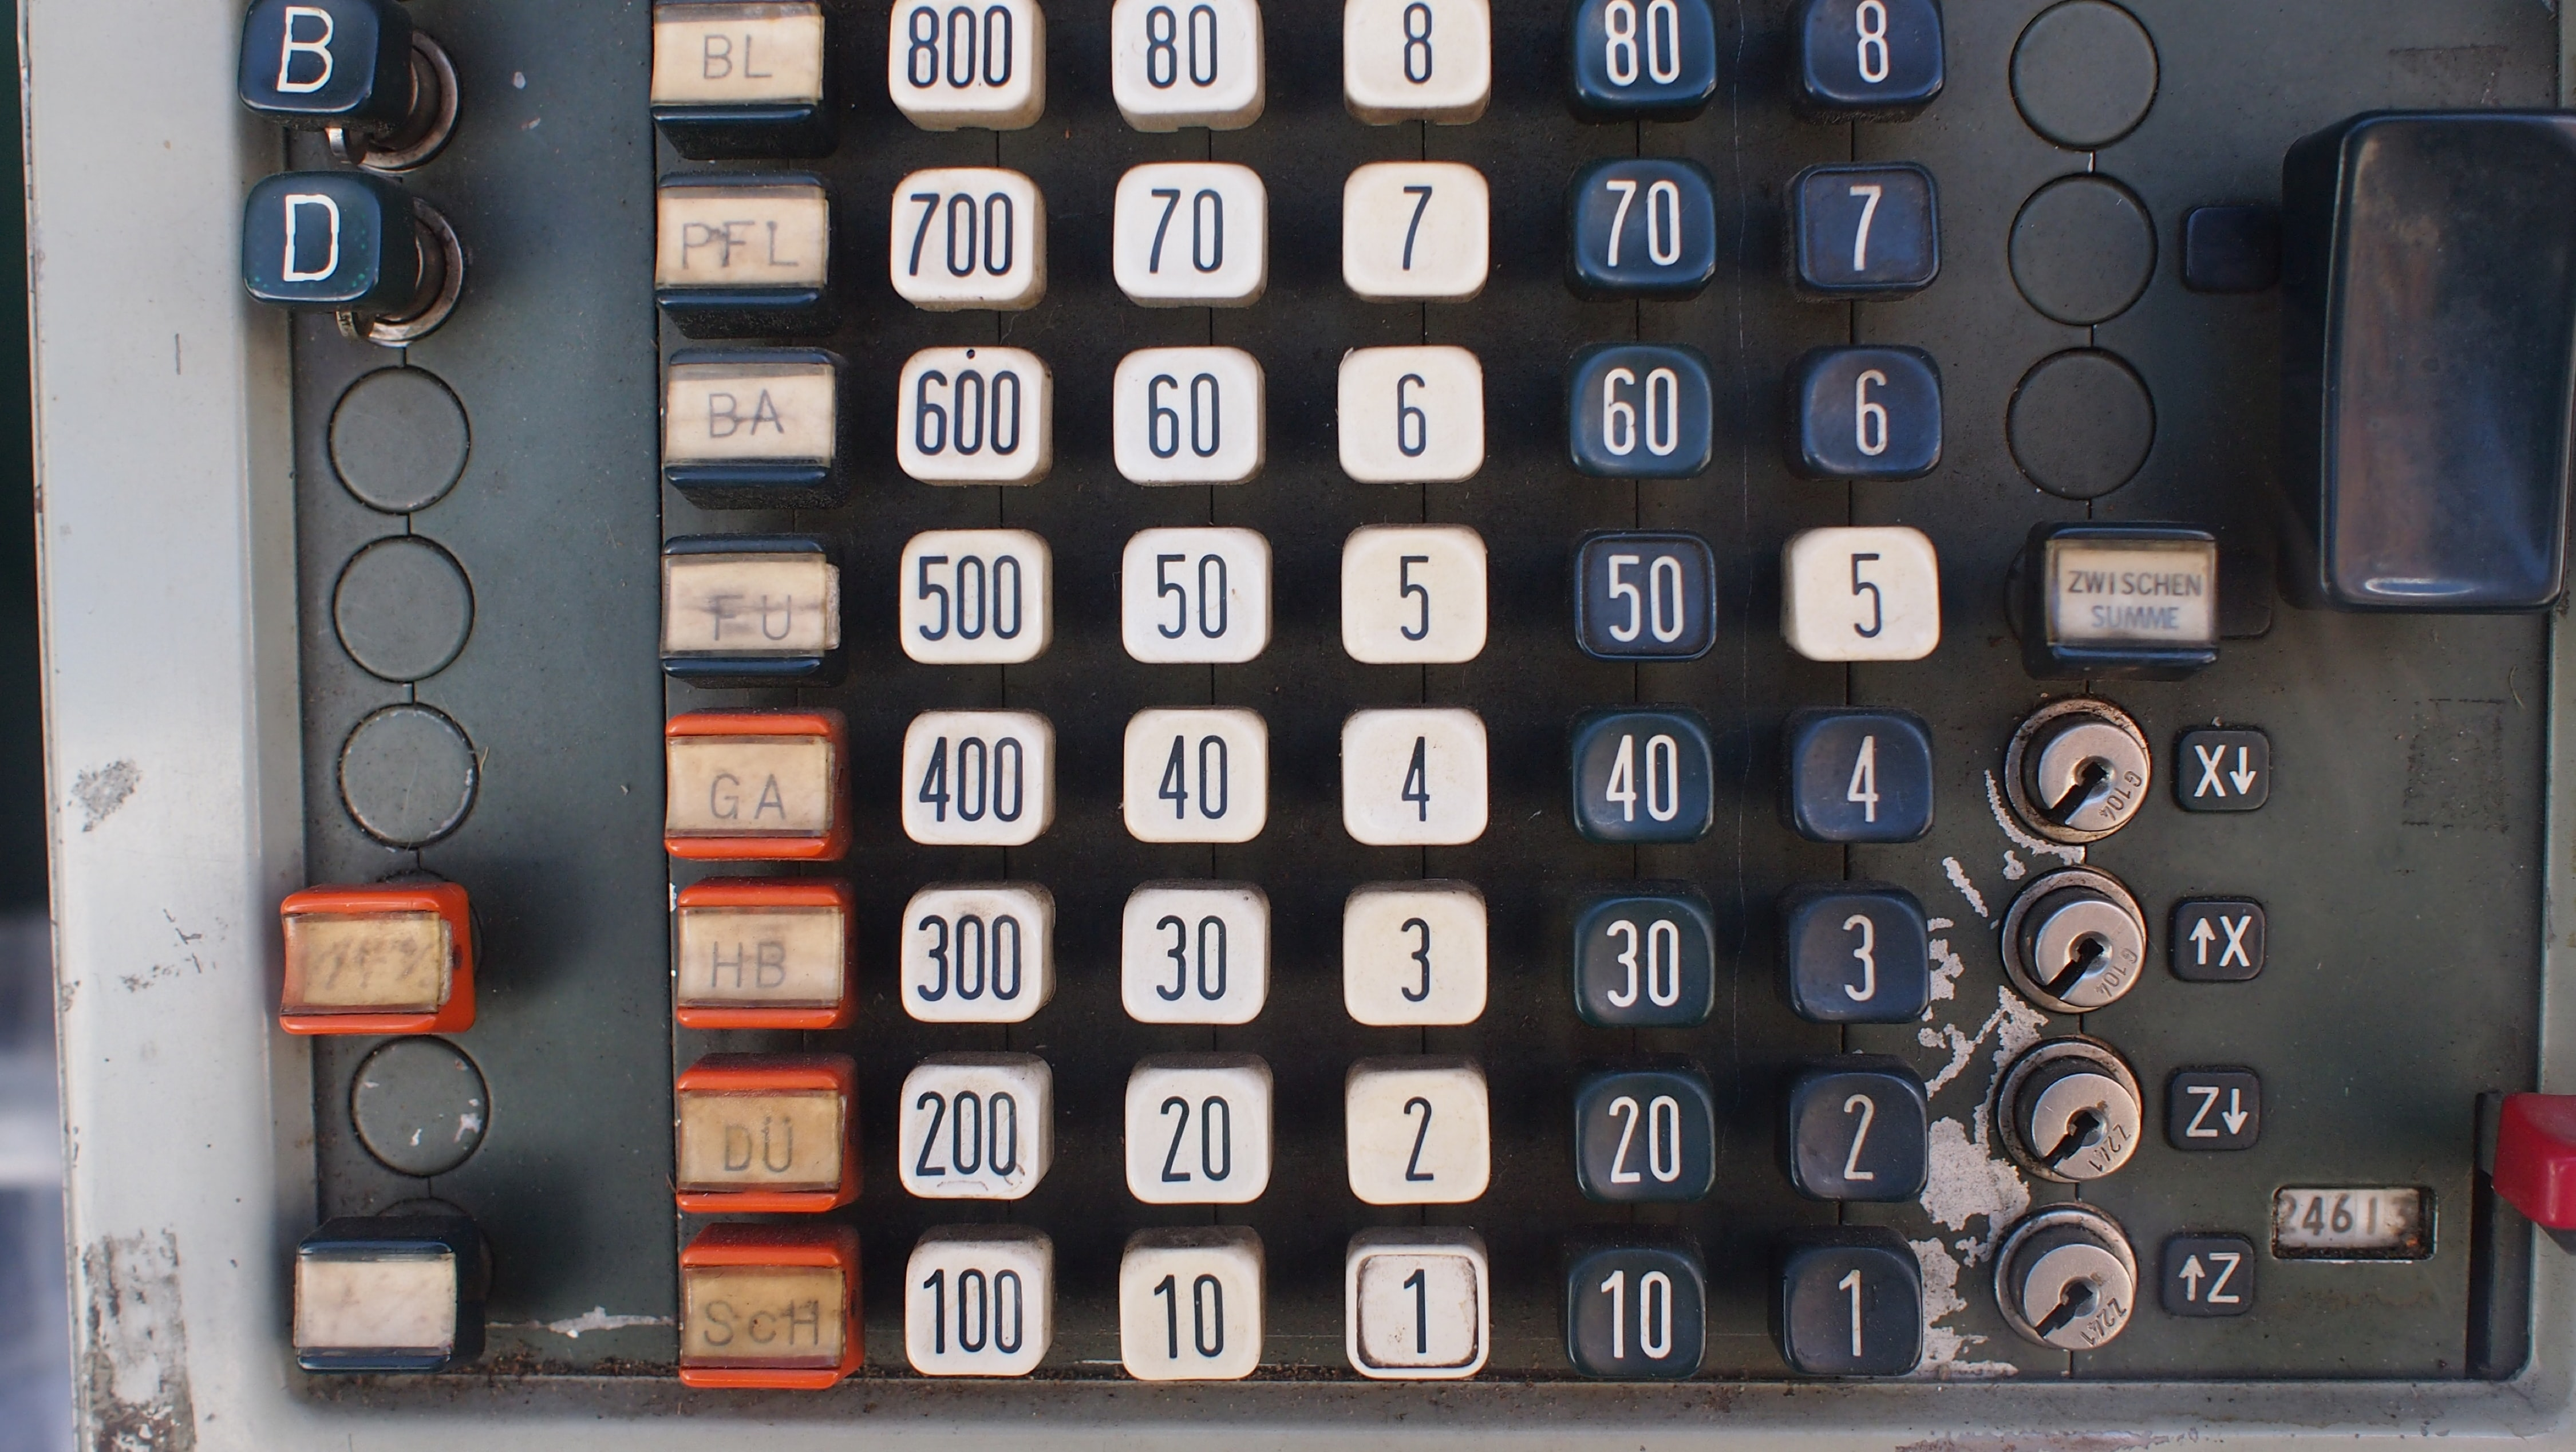
\includegraphics[width=\textwidth]{images/oldcomp.jpg}
	\end{center}
	\begin{flushright}
		\textit{(Bruno Neurath-Wilson)}
	\end{flushright}
	
	\end{frame}

	\begin{frame}{Historické náhledy na software}
		\begin{description}
			\item[1950-60]
			  \begin{itemize}
			  	\item software jako předmět \textbf{výzkumu}
			  	\item software jako součást hardware
			  	\item \textbf{otevřenost a spolupráce} mezi univerzitami a korporacemi
			  	\item \textbf{monetizace nebyla} cílem
			  	\item často šířen jako \textbf{veřejný statek} (public-domain)
			  	\item \textbf{dostupný zdrojový kód}
			  \end{itemize}
		\end{description}
	\end{frame}

	\begin{frame}{Historické náhledy na software}
	\begin{description}
		\item[1961-70]
		\begin{itemize}
			\item \textbf{rozvoj} programovacích jazyků a kompilerů
			\item \textbf{přibalený} (bundled) vs. samostatný software
			\item rozvoj specializovaného softwaru nezávislého na hardware
			\item neochota zákazníků \textbf{platit} za software \textbf{dvakrát}
			\item soudní spor \textbf{USA vs. IBM (1969)} -- přibalování software poškozuje konkurenci
			\item software poskytován s různými \textbf{omezeními}
		\end{itemize}
	\end{description}
	\end{frame}

	\begin{frame}{Historické náhledy na software}
	\begin{description}
		\item[1971-80]
		\begin{itemize}
			\item změna obchodních modelů -- např. OS zdarma, ale placené \uv{patche}
			\item poprvé tzv. \textbf{vendor lock-in}
			\item soudní rozhodnutí z roku 1974 uznalo software za \textbf{chránitelný copyrightem} (copyrightable)
			\item software jako licencovaný produkt
			\item \textbf{konec distribuce zdrojových kódů}, distribuován je pouze tzv. \textbf{strojový} (machine) kód
			\item \textbf{patentová ochrana} softwarových řešení
		\end{itemize}
	\end{description}
	\end{frame}

	\begin{frame}{Historické náhledy na software}
	\begin{description}
		\item[1981-90]
		\begin{itemize}
			\item touha po původní myšlence \textbf{sdílení} však nadále existuje mezi \textbf{hobíky} a \textbf{hackery}
			\item vznik online sdílených komunit (např. tzv. BBS)
			\item Richard Stallman a vznik projektu \textbf{GNU} (1983)
			\item \textbf{Free Software Manifesto} a vznik \textbf{Free Software Foundation} (1985)
			\item GNU General Public License (1989)\footnote{Dneska již ve třetím vydání.}
			\item jádro projektu GNU -- \textbf{Hurd}
		\end{itemize}
	\end{description}
\end{frame}

	\begin{frame}{Historické náhledy na software}
	\begin{description}
		\item[1991-dosud]
		\begin{itemize}
			\item jádro \textbf{Linux} (na bázi Minix) od Linuse Torvaldse pod licencí GPL
			\item přidala se \textbf{komunita vývojářů} a projekt začal růst
			\item spojení GNU projektu s linuxovým jádrem -- \textbf{GNU/Linux}
			\item Debian -- důraz na principy FSF
			\item některé \textbf{části} jádra \textbf{nesplňují} definici \textit{free software}
			\item mnoho dalších distribucí a projektů založených na GNU/Linux
		\end{itemize}
	\end{description}
\end{frame}
	
	\begin{frame}{Svobodný software}
		\begin{center}
			\includegraphics[width=\textwidth]{images/code.jpg}
		\end{center}
		\begin{flushright}
			\textit{(Chris Ried)}
		\end{flushright}
	\end{frame}
	
	\begin{frame}{Co je Svobodný software?}
		\textit{Svobodný software} je takový, který zaručuje svým uživatelům \textbf{čtyři základní svobody}.
				\begin{itemize}
			\item právo spouštět program, jak si přejete a za jakýmkoliv účelem
			\item právo zkoumat, jak program funguje, a právo upravit si jej libovolně pro své účely (otevřený kód)
			\item právo šířit kopie, abyste pomohli ostatním
			\item právo šířit vámi modifikované verze programu a umožnit komunitě, aby těžila z vašich vylepšení (otevřený kód)
		\end{itemize}
	\end{frame}

	\begin{frame}{Právo spouštět}
		\begin{itemize}
			\item uživatel smí program \textbf{spouštět za jakýmkoliv} účelem
			\item není důležité, za jakým \textbf{účelem byl program vytvořen}
			\item právo spouštět \textbf{nezakládá nároky na funkčnost} programu
		\end{itemize}
    \end{frame}	

	\begin{frame}{Právo zkoumat a měnit}
	\begin{itemize}
		\item uživatel smí program studovat -- k tomu je nutné, aby měl tzv.~\textbf{otevřený kód} (open source).
		\item uživatel si smí program upravit pro svou vlastní potřebu, jakožto i pro kohokoliv jiného a \textbf{není povinen žádat o svolení}
		\item uživatel má právo volně spouštět \textbf{své vlastní modifikace programu}
		\item uživatel má právo k programu připojovat další \textbf{svobodné knihovny, funkce, a moduly}
	\end{itemize}
	\end{frame}	

	\begin{frame}{Právo šířit}
	\begin{itemize}
		\item uživatel má právo \textbf{šířit kopie programu zdarma nebo za úplatu} a nemusí nikoho žádat o svolení ani nikomu za toto právo platit
		\item uživatel má právo program modifikovat \textbf{sám pro sebe nebo pro kohokoliv jiného}. Pokud změny zvěřejníte, nejste povinni toto nikomu hlásit
		\item uživatel má právo \textbf{své vlastní modifikace} vydat pod jakoukoliv licencí (program přestane být \textit{free})
		\item uživatel má právo distribuovat \textbf{zdrojové i binární} kopie programu.
	\end{itemize}
	\end{frame}	

	\begin{frame}{Kopírování zabíjí}
	\begin{center}
		
\includegraphics[width=\textwidth]{images/cc.jpg}
	\end{center}
	\begin{flushright}
		\textit{(Umberto)}
	\end{flushright}
	\end{frame}

	\begin{frame}{Copyright}
	\textbf{Copyright} je způsobem, jak autorovi zajistit jeho práva k~vytvořeným dílům.
	\begin{itemize}
		\item primárně zakazuje komukoliv cokoliv
		\item použití jenom se svolením autora
		\item většinou za úplatu (tantiémy)
	\end{itemize}
	\end{frame}	

	\begin{frame}{Copyleft}
	\textbf{Copyleft} je způsobem, jak zaručit všem svobodu a práva při používání programů.
	\begin{itemize}
		\item není opakem slova \textbf{Copyright}, naopak je postaven na \textbf{Copyrightu}.
		\item nemá za účel zpochybnit autorství
		\item vyžaduje, aby modifikace a redistribuce programu poskytovaly všechna práva, která program poskytoval předtím
		\item dává volnost programátorům
		\item chrání programy před \textbf{proprietarizací}
		\item toto je zaručeno správnou licencí
	\end{itemize}
\end{frame}	

	\begin{frame}{Veřejné použití (public-domain)}
		Držitelé práv (copyright) dovolují použít svůj kód jakkoliv i bez uvedení jejich autorství.
	\end{frame}	
	
	\begin{frame}{Volná licence (permissive)}
		Držitelé práv (copyright) dovolují použít svůj kód jakkoliv, i v~proprietárním použití, pokud budou uvedeni dále jako autoři kódu.
	\end{frame}	
	
	\begin{frame}{Slabý copyleft}
	   Držitelé práv (copyright) sdílejí kód za předpokladu, že lidé, kteří dělají změny do jádra projektu dále předávají toto stejné právo na uživatele.
	\end{frame}	

	\begin{frame}{Silný copyleft}
	Držitelé práv (copyright) sdílejí kód za předpokladu, že lidé, použijí tento kód v jakémkoliv odvozeném díle, i pouhým nalinkováním, předají toto stejné právo na uživatele.
	\end{frame}	

	
\begin{frame}{Licence vyhovující definici svobodného software}
	\begin{itemize}
		\item \textbf{GNU General Public License (GPL)}
		\item GNU Lesser General Public License (LGPL)
		\item Apache License 2.0
		\item Berkely Database License
		\item Modified BSD
		\item Perl 5 License
		\item X11 License
		\item a mnoho dalších\footnote{https://www.gnu.org/licenses/license-list.html}
	\end{itemize}
\end{frame}

\begin{frame}{Proč některé licence nevyhovují?}
	Protože chrání \textbf{příliš málo} nebo naopak \textbf{příliš mnoho}.
\end{frame}

	\begin{frame}{Zavřeno!}
	\begin{center}
		\includegraphics[width=\textwidth]{images/closed.jpg}
	\end{center}
	\begin{flushright}
		\textit{(David Clode)}
	\end{flushright}
\end{frame}

\begin{frame}{Problémy vyplývající z proprietární licence}
	\begin{itemize}
		\item náklady na pořízení
		\item uživatelská podpora
		\item zabezpečení
		\item úprava podle přání zákazníka
		\item vendor lock-in
		\item možné odchýlení od standardů
		\item softwarové patenty
	\end{itemize}
\end{frame}

\begin{frame}{Náklady na pořízení}
	\begin{itemize}
		\item jednorázové (licence)
		\item opakované (předplatné)
		\item kombinované
		\item riziko počítačového pirátství
	\end{itemize}
\end{frame}

\begin{frame}{Uživatelská podpora}
	\begin{itemize}
		\item často zanedbávaná
		\item mnohdy podfinancovaná
		\item leckde outsourcing některých úrovní podpory
		\item obtížně dostupná
	\end{itemize}
\end{frame}

\begin{frame}{Zabezpečení}
	\begin{itemize}
		\item neprostá nemožnost zjistit, jak software s bezpečností zachází
		\item riziko neobjevených chyb
		\item riziko přeprodávání uživatelských dat třetím stranám
		\item riziko ovlivňování chování uživatelů
	\end{itemize}
\end{frame}

\begin{frame}{Úprava podle přání zákazníka}
	neboli \textbf{customizace} (customization)
	\begin{itemize}
		\item nelze nechat zákaznicky upravit
	\end{itemize}
\end{frame}

\begin{frame}{Vendor lock-in}
	aneb \textbf{závislost zákazníka na produktu} a nemožnost úniku
	
	\begin{itemize}
		\item firma se vybaví proprietárním řešením
		\item po čase řešení přestane vyhovovat
		\item data nejsou jednoduše přenositelná jinam
		\item formát není dobře zdokumentován
		\item migrace na jiný produkt finančně a časově náročná
		\item kompatibilita mezi spolupracujícími firmami nejasná
		\item plánované zastarávání (planned obsolescence)
	\end{itemize}
\end{frame}

\begin{frame}{Standardy}
	\textbf{Standardy} definují přístup k řešení konkrétních IT problémů.
 	 	
	\begin{itemize}
		\item kompatibilita napříč počítačovým světem
		\item svoboda volby
	\end{itemize}
	V proprietárních systémech nejsou často respektovány a to způsobuje mnoho problému.
	\begin{itemize}
		\item nerespektování $=$ konkurenční výhoda
		\item bludný kruh pro uživatele (vendor lock-in)
		\item nutnost synchronizace mezi uživateli
		\item revolvingové náklady na používání
	\end{itemize}
\end{frame}

\begin{frame}{Softwarové patenty}
	\begin{itemize}
		\item chrání \textbf{duševní vlastnictví} autora
		\item nutnost zakoupit licenci na jejich použití (drahé)
		\item ochrana vlastního produktu
		\item nedostupnost produktu
		\item zpomalení nebo zastavení vývoje
	\end{itemize}
\end{frame}

\begin{frame}{Příklady proprietárních řešení}
	Které z následujících jste již viděli naživo?
\begin{itemize}
	\item Auto s kapotou, která se nedá otevřít jinak než v servisu.
	\item Mobilní telefon s baterií uvnitř těla a chráněnou plombou.
	\item Lyže s vázáním, jehož velikost nelze přizpůsobit velikosti boty.
	\item Kávovar se specifickým tvarem kapslí.
	\item Písnička ve formátu, který lze přehrát pouze na konkrétním zařízení.
\end{itemize}
Myslíte, že takové výrobky nám prospívají?
\end{frame}

	\begin{frame}{Ze tmy do světla}
	\begin{center}
		
\includegraphics[width=9cm]{images/opened.jpg}
	\end{center}
	\begin{flushright}
		\textit{(Matthew T. Rader)}
	\end{flushright}
	\end{frame}

\begin{frame}{Výhody sdílení a otevřeného kódu 1}
	\begin{itemize}
		\item žádný vendor lock-in
		\item dodržování průmyslových standardů
		\item vliv na směřování technologického vývoje
		\item udržení tempa s konkurencí
		\item vyšší vliv organizací
		\item vyšší kvalita kódu
		\item rychlajší vývoj lepšího softwaru
		\item vyšší spolehlivost a bezpečí
	\end{itemize}
\end{frame}

\begin{frame}{Výhody sdílení a otevřeného kódu 2}
	\begin{itemize}
		\item lepší zachycení potenciálních bezpečnostních hrozeb
		\item přímá interakce s uživateli
		\item vývoj a inovace společně s komunitou
		\item udržení tempa s konkurencí
		\item rychlejší schopnost reakce na trh
		\item přilákání a udržení talentů
		\item uvědomění si změn ve vývoji projektu
		\item různé pohledy na vývoj
		\item poskytnutí rámce pro spolupráci
	\end{itemize}
\end{frame}

\begin{frame}{Obchodní modely na bází otevřeného kódu}
	Podle Wikipedie\footnote{https://en.wikipedia.org/wiki/Business\_models\_for\_open-source\_software}:
 \begin{itemize}
		\item kód není předmětem prodeje
		\item prodej uživatelů
		\item předprodej kódu
		\item prodej intelektuálního vlastnictví
		\item prodej proprietárních doplňků
		\item jiné
 \end{itemize}
\end{frame}

\begin{frame}{Kód není předmětem prodeje}
	\begin{itemize}
		\item služby
		\item značkový \textit{merch}
		\item Software-as-a-Service (SaaS)
		\item dobrovolné dary
		\item crowdsourcing
	\end{itemize}
\end{frame}

\begin{frame}{Prodej uživatelů}
	\begin{itemize}
		\item partnerství s organizací (Google Summer of Code)
		\item reklama
	\end{itemize}
\end{frame}

\begin{frame}{Předprodej kódu}
	\begin{itemize}
		\item vývoj podle odměny (funkce, které si někdo zaplatí mají přednost)
		\item placená předobjednávka nebo ukázka (preview)
	\end{itemize}
\end{frame}

\begin{frame}{Prodej duševního vlastnictví}
	\begin{itemize}
		\item Dvojí licence neboli \textit{otevřené jádro} (zadarmo pro hobíky, placené pro firmy)
		\item Prodej certifikací a obchodní značky (trademark)
		\item Přelicencování na proprietární software (u licencí, které to dovolují)
	\end{itemize}
\end{frame}

\begin{frame}{Prodej doplňků}
	\begin{itemize}
		\item proprietární doplňky (moduly, pluginy)
		\item prodej proprietárních částí softwarového produktu
		\item prodej proprietárních updatovacích systémů
	\end{itemize}
\end{frame}

\begin{frame}{Pečeme piškoty proprietárně}
	\begin{enumerate}
		\item Upečeme piškoty.
		\item Zabalíme je.
		\item Označíme značkou.
		\item Prodáme je.
	\end{enumerate}
\end{frame}

\begin{frame}{Pečeme piškoty otevřeně}
	\begin{enumerate}
		\item Upečeme piškoty.
		\item Zabalíme je.
		\item Označíme značkou.
		\item \textbf{Na obal vytiskneme návod na pečení piškotů, naše poznámky, a nejlepší pečící postupy.}
		\item Prodáme je.
	\end{enumerate}
\end{frame}

\begin{frame}{Podporujeme 4 základní práva.}
	\begin{enumerate}
		\item Použij.
		\item Prostuduj.
		\item Změň.
		\item Sdílej.
	\end{enumerate}
\end{frame}

\begin{frame}{Každý peče svoje piškoty}
	ale pouze za předpokladu, že $\ldots$
	\begin{itemize}
		\item dodržuje nařízení o zdraví a bezpečnosti a další zákony
		\item sdílí svoje úpravy piškotů s komunitou pekařů, chce-li je prodávat
		\item souhlasí, že komunitu pekařů nebude vinit za jakékoliv následky, které pečení piškotů může mít.
	\end{itemize}
\end{frame}

\begin{frame}{Proč je dobré recept sdílet?}
	\begin{itemize}
		\item zlepšování receptu a výroba lepších piškotů v globální spolupráci pekařů
		\item identifikace možných variací receptu vhodných pro menší trhy, o kterých jste sami nepřemýšleli
		\item vytvoření komunity pekařů, kteří podporují a šíří váš recept
		\item objevte talentované pekaře, které můžete zaměstnat ve vašem obchodě
		\item umístěte se jako čelní výrobce piškotů podle vašeho receptu
	\end{itemize}
\end{frame}

	\begin{frame}{Sharing is caring}
	\begin{center}
		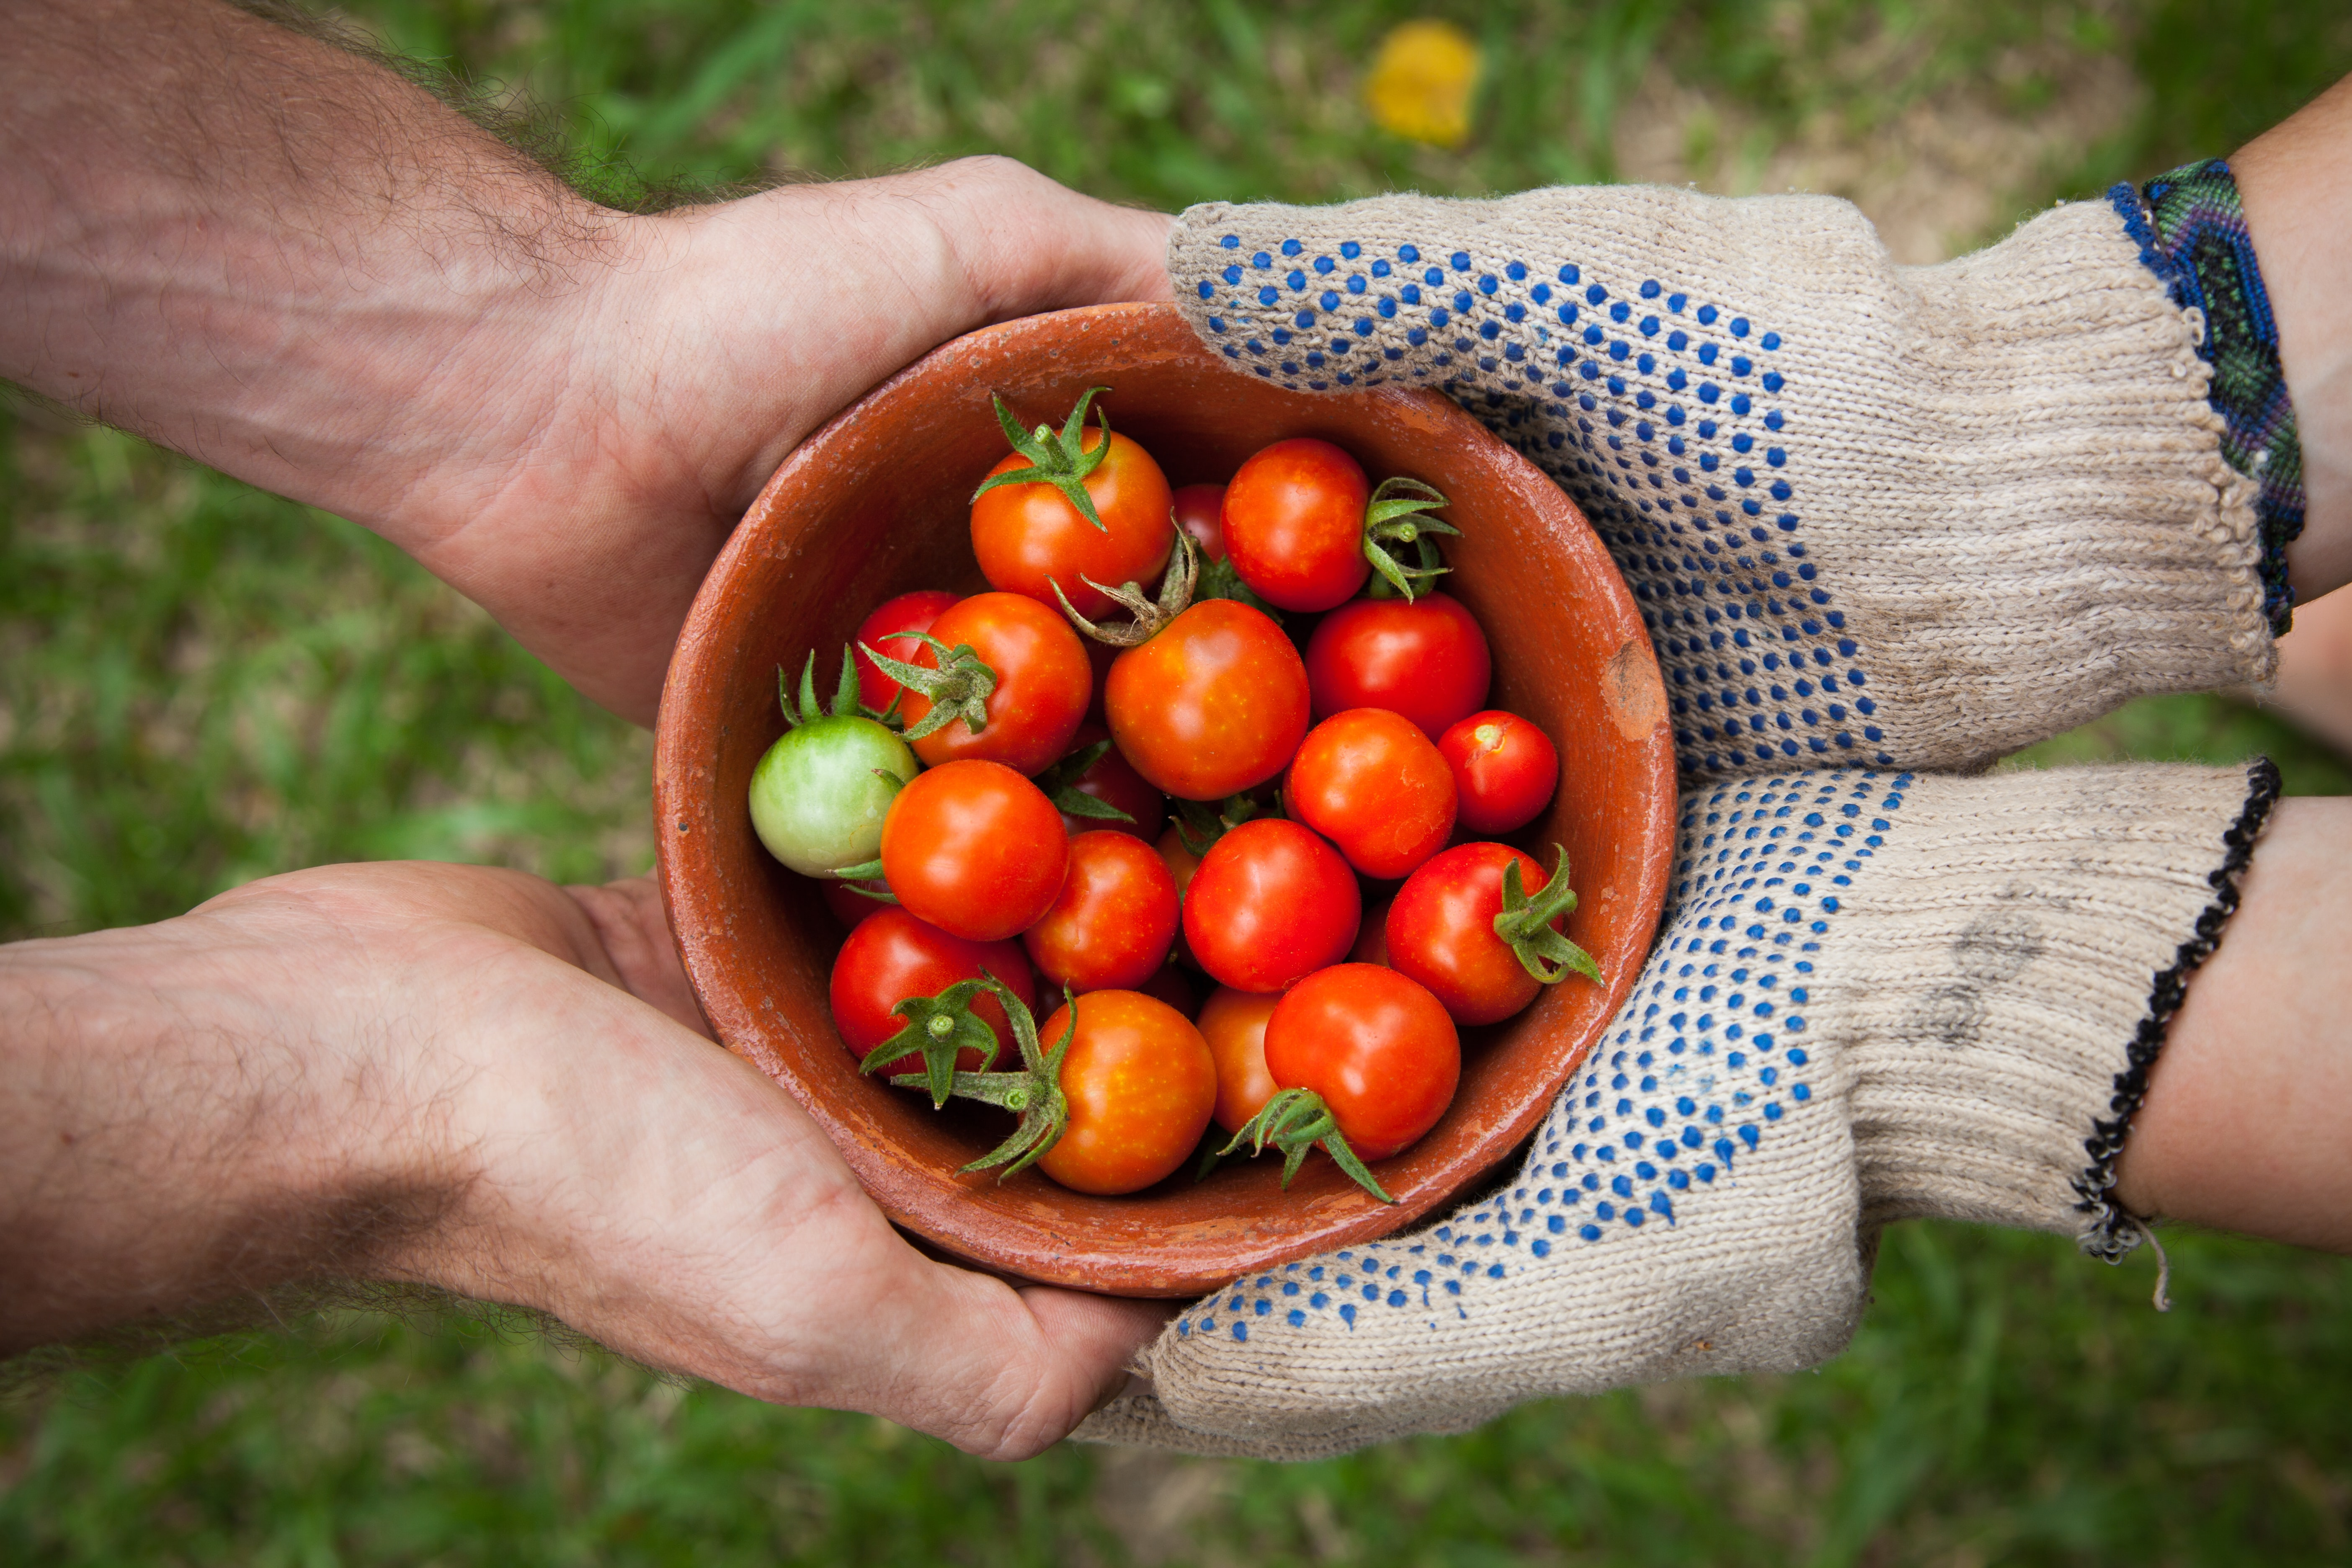
\includegraphics[width=\textwidth]{images/share.jpg}
	\end{center}
	\begin{flushright}
		\textit{(Elaine Casap)}
	\end{flushright}
\end{frame}

	\begin{frame}{Někdo nějaké otázky?}
	\begin{center}
		
\includegraphics[width=\textwidth]{images/questions.jpg}
	\end{center}
	\begin{flushright}
		\textit{(Camylla Battani)}
	\end{flushright}
	\end{frame}

\begin{frame}{Kredit}
	Vytvořeno s použitím:
	\begin{itemize}
		\item operačního systému \textbf{Fedora Workstation 32}
		\item programu \textbf{\TeX{studio}}
		\item typografického systému \textbf{\LaTeXe}
		\item obrázků ze serveru \textbf{unsplash.com}
	\end{itemize}
	To vše díky free software a ochotě lidí sdílet.
\end{frame}

\begin{frame}
	\begin{center}
		{\Huge Děkuji za pozornost!}
	\end{center}
\end{frame}

\end{document}